\documentclass{article}
\usepackage{graphicx}
\usepackage{hyperref}
\hypersetup{
  colorlinks   = true,    % Colours links instead of ugly boxes
  urlcolor     = blue,    % Colour for external hyperlinks
  linkcolor    = blue,    % Colour of internal links
  citecolor    = red      % Colour of citations
}

\title{UT Quantum Collective}
\begin{document}
\maketitle{}

\tableofcontents

\begin{abstract}
	We are a community where undergraduate students engage with each other to learn and research topics about everything Quantum.
\end{abstract}

\subsection{What we Do}
	We hold weekly meetings for research groups who go out and invesitgate topics, learning labs where we teach computing with Qiskit (a quantum circuit compiler), and reading groups where we journey through interesting papers.

	In addition, we host semesterly quantum hackathons, occasional guest speakers, and collaborate with other university quantum clubs to host the global SQUID conference.

	Join \href{https://discord.gg/UBnRaHuzF9}{our Discord space} to see everything that's going on.

	\subsection{Cool Pictures}

	todo: Add pictures of us. idk where to get them

% Cool IBM pictures at https://www.flickr.com/photos/ibm_research_zurich/40645906341/in/photostream/
%Picture from https://nanoscience.oxinst.com/products/proteoxmx
	\begin{figure}[h!]
		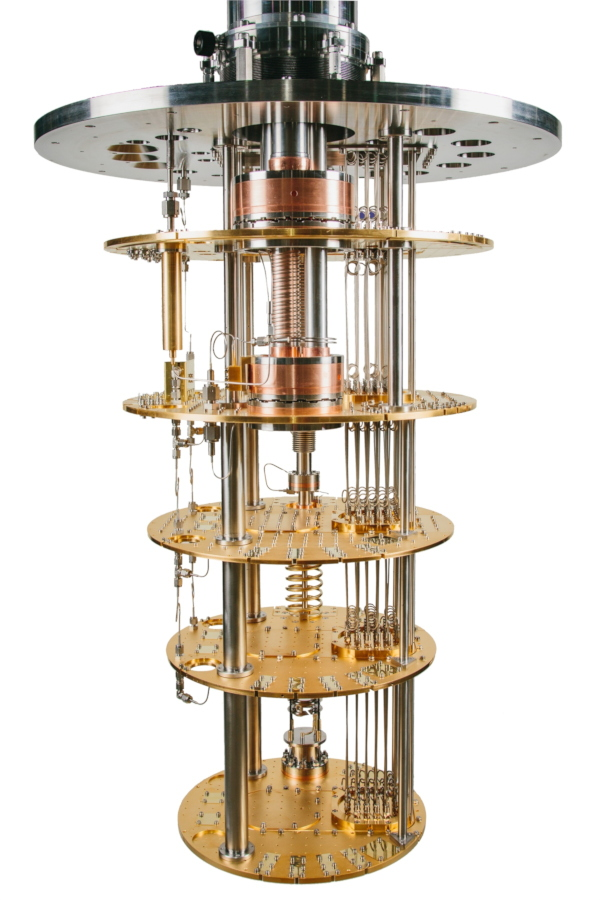
\includegraphics[height=160px]{dilutionfridge_small.jpg}
		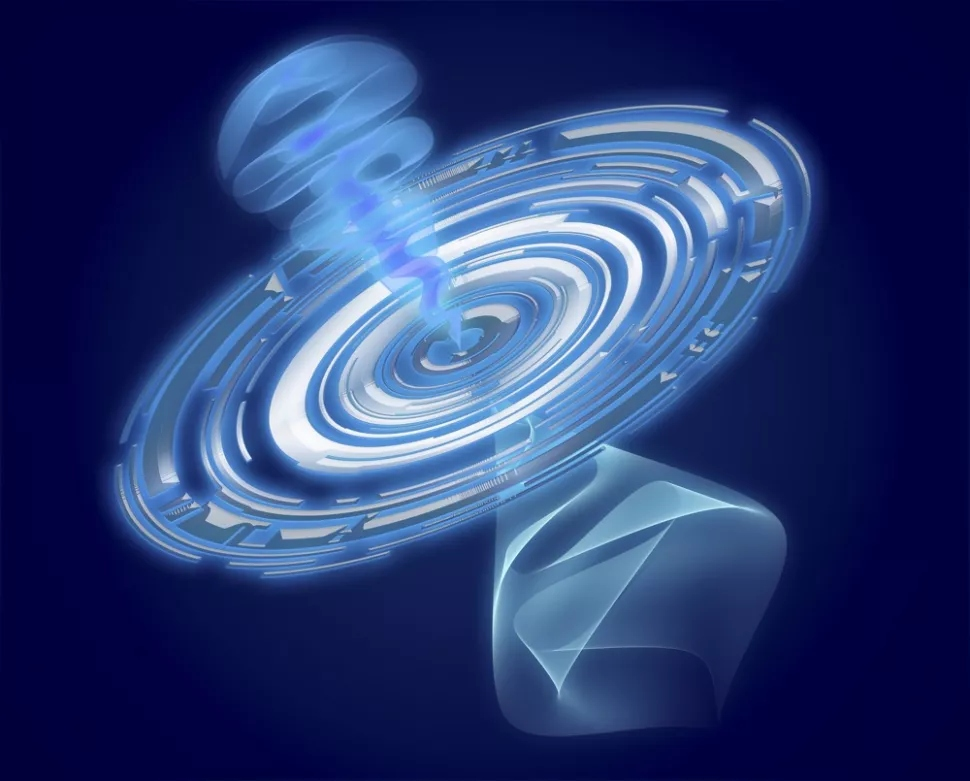
\includegraphics[height=160px]{real_qubit.jpg}
		\caption{These are what quantum computers really look like}
	\end{figure}


	\subsection{Meet the Dirac-tors}

	todo

	\subsection{See Also}

	\begin{itemize}
		\item Email: \href{mailto:qdiractor@gmail.com}{qdiractor@gmail.com}
		\item \href{https://discord.gg/UBnRaHuzF9}{Discord}
		\item \href{https://www.instagram.com/texasquantum/?hl=en}{Instagram}
		\item \href{https://utexas.campuslabs.com/engage/organization/quantum-collective}{Hornslink (Become a Member!)}
	\end{itemize}

\section{Resources}

\subsection{Learning}
\begin{itemize}
	\item \href{https://www.thomaswong.net/introduction-to-classical-and-quantum-computing-1e3p.pdf}{Thomas Wong's textbook} is an introductory book which takes the time to give you the foundations in classical computing before teaching you quantum computing.

	\item \href{https://www.qisforquantum.org/}{Q is for Quantum} I haven't looked at this one, but I probably should before I put it here.
	
	\item \href{https://qiskit.org/}{Qiskit} has a series of tutorials on creating quantum circuits and a library to run them.

	\item Scott Aarronson's \href{https://www.scottaaronson.com/qclec.pdf}{QIS I} and \href{https://www.scottaaronson.com/qisii.pdf}{QIS II} lecture notes. 
\end{itemize}

\subsection{In the Field}
\begin{itemize}

	\item \href{https://arxiv.org/list/quant-ph/new}{arXiv} is the place where all papers are published before they get approved by journals

	\item \href{https://scirate.com/arxiv/quant-ph?range=14}{SciRate} is an arXiv wrapper which quantum researchers use to upvote and comment on the most cutting edge papers.

	\item \href{https://quantum-computing.ibm.com/}{IBM's Quantum Experience} contains a graphical quantum circuit builder and idk what else, I'll have to look at this one too.

	\item \href{https://www.quantumgrad.com/}{Quantum Grad} has articles and information on internship and research opportunities.
\end{itemize}

\subsection{Community}
\begin{itemize}
		

	\item \href{https://scottaaronson.blog/}{Scott Aaronson's blog}

	\item \href{https://quantumfrontiers.com/}{Quantum Frontiers} is a blog by the Institute for Quantum Information and Matter @ Caltech
\end{itemize}

\section{Archives}

We have recordings of past learning labs, guest speakers, and events on \href{https://www.youtube.com/@quantumcollective_UT}{our Youtube Channel}

\section{\href{https://discord.gg/UBnRaHuzF9}{Discord}}

\begin{figure}[h!]
	\centering
	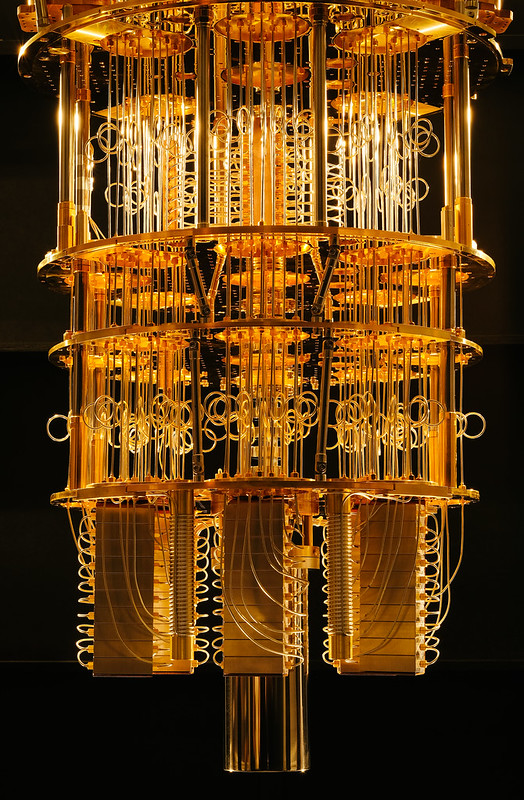
\includegraphics[width=\linewidth]{darktheme_fridge_medium.jpg}
\end{figure}
\end{document}

